\hypertarget{vancouver-entre-mer-et-montagne}{%
\section{Vancouver, entre mer et
montagne}\label{vancouver-entre-mer-et-montagne}}

Quittant les latitudes méso-américaines, nous arrivons à Vancouver
pleins de curiosité. Quelle est donc cette ville qui revient si souvent
dans les classements des ville les plus agréables du monde ? Nous avons
eu le bonheur de le découvrir à travers l'accueil généreux de Rola,
Andrew et de leurs trois garçons. L'art de vivre à Vancouver c'est la
proximité à la mer, le charme des montagnes si proches et le plaisir de
partir en ferry sur les petites îles situées dans le détroit.

Voici une petite carte pour mieux repérer les lieux :

\hypertarget{mapid}{}

\emph{Downtown Vancouver}, c'est la ville de béton, d'acier et de verre.
Moderne, mais agréable à la marche, avec des petits commerces à tous les
coins de rue. On y a même trouvé un
\href{/manger-au-liban.html}{restaurant libanais} qui fait d'excellentes
\emph{manoushé}. On trouve un peu de tout dans la ville, des quartiers
originels de la ville comme \emph{Gastown}, aux quartiers cossus dans
lesquels on s'arrache des propriétés de millionnaires comme à
\emph{Shaughnessy}. L'un des marqueurs visibles de l'attractivité de la
ville, c'est la présence de citoyens canadiens d'origine chinoise (et
surtout des multiples pancartes en chinois), ce qui s'explique par
l'immigration importante qui a précédé le rattachement de Hong-Kong à la
Chine continentale en 1997. Certains quartiers sont particulièrement
agréables à explorer, notamment le tour en vélo de \emph{Stanley Park},
superbe moment de notre visite, ou encore \emph{Granville Island},
presqu'île où l'artisanat et les spécialités culinaires locales
abondent.

\begin{figure}
\centering
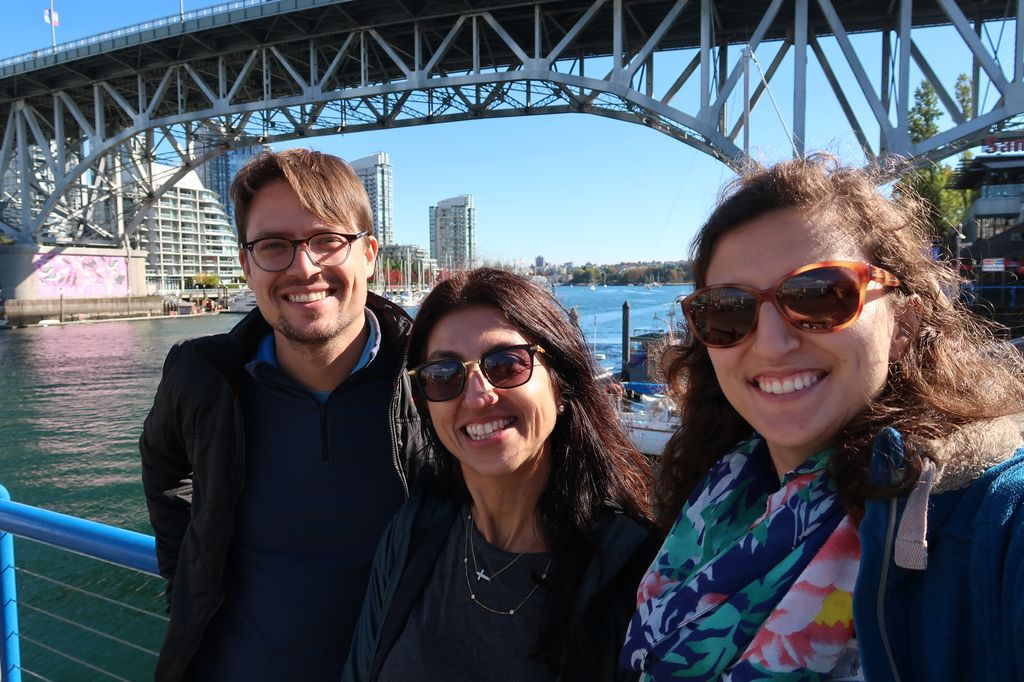
\includegraphics{images/20181016_granville.JPG}
\caption{Notre hôte de choc, Rola, et nous à Granville Island.}
\end{figure}

Mention spéciale également à l'Université de Colombie Britannique (UBC),
située sur un très beau territoire boisé à l'ouest de la ville. Nous
avons suivi la visite guidée destinée aux futurs étudiants et avons été
bluffé par la qualité de l'accueil. Ça donne vraiment envie de retourner
aux études !

\begin{figure}
\centering
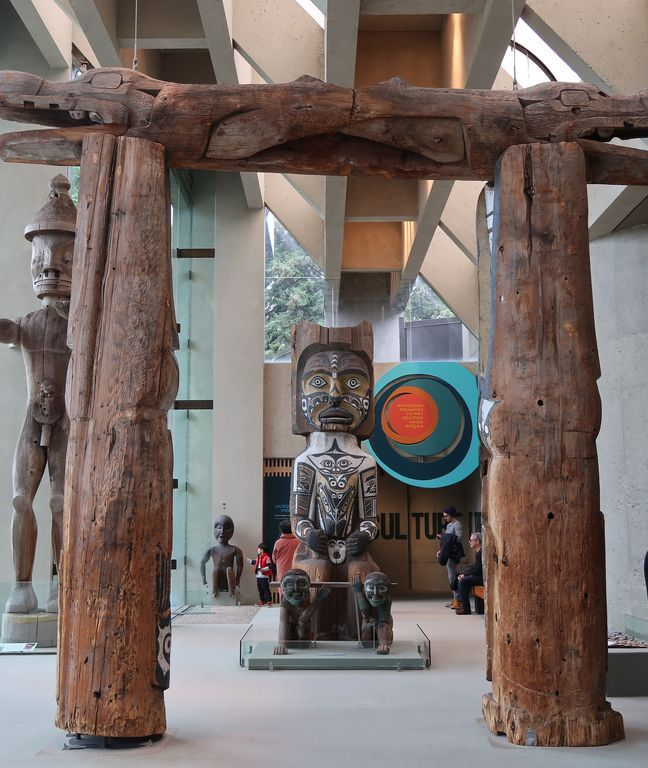
\includegraphics{images/20181016_ubc.JPG}
\caption{Et en plus, l'UBC dispose d'un formidable musée d'anthropologie
où l'on peut admirer ces totems typiques de la côte ouest.}
\end{figure}

Nous avons passé deux semaines dans le quartier de West Vancouver, l'un
des quartiers huppés de la ville. Comme je le disais en introduction,
nous avons eu beaucoup de plaisir à partager la vie quotidienne d'une
famille de cinq personnes très occupées (et nous avons eu la chance
d'avoir Rola pour guide quasiment tous les jours !). L'un des moments
forts a été le fête de Thanksgiving \emph{canadien} (dont nous ne
connaissions pas l'existence avant ça !).

\begin{figure}
\centering
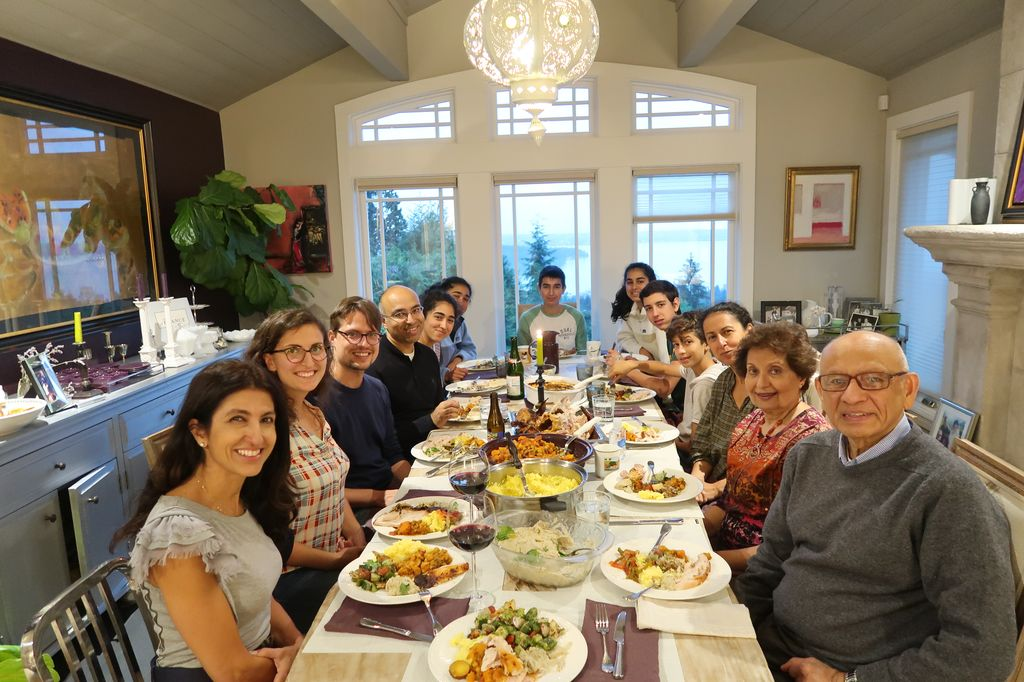
\includegraphics{images/20181016_thanksgiving.JPG}
\caption{La table était pleine !}
\end{figure}

Mais ce qui fait le charme de Vancouver c'est la proximité à la nature.
Entre le \emph{Grouse grind}, que les locaux pratiquent le chronomètre à
la main et les nombreux sentiers dans les parcs qui jouxtent la ville,
nous n'avons pas été déçus. Whistler, la station de sports d'hiver où
ont eu lieu les jeux olympiques d'hiver de 2010 est une autre belle
destination, à une heure de voiture à peine du centre ville. On peut y
randonner à loisir, à pied ou en vélo (le ski c'est pour plus tard dans
l'année).

\begin{figure}
\centering
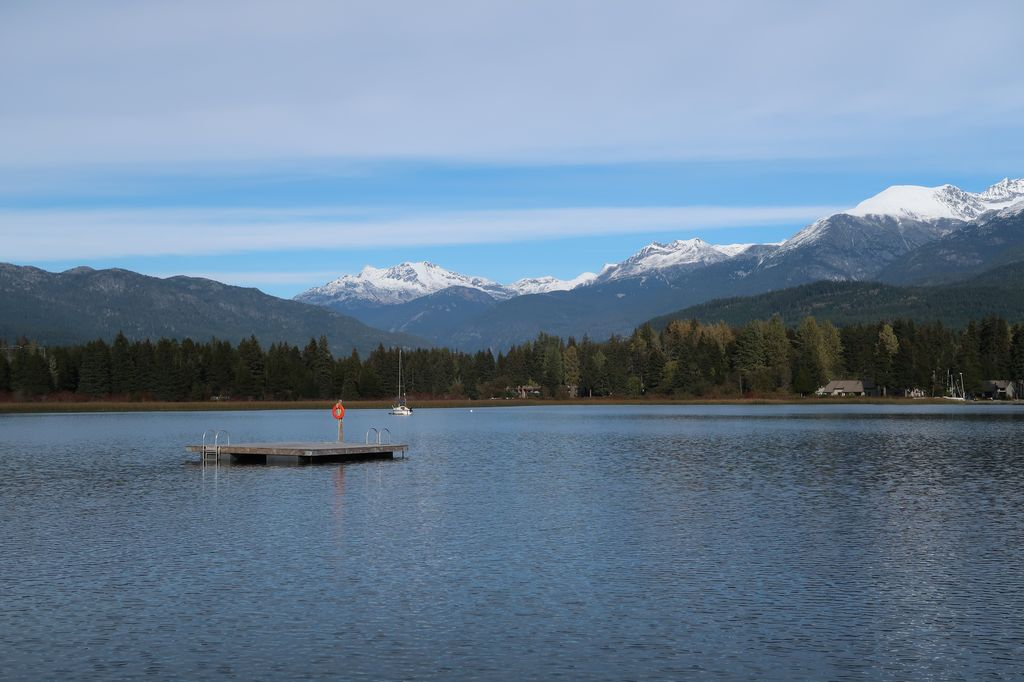
\includegraphics{images/20181016_whistler.JPG}
\caption{La neige nous regarde depuis les sommets autour de Whistler.}
\end{figure}

Nous avons aussi eu le plaisir de passer une nuit dans un \emph{cottage}
sur la \emph{Sunshine Coast}. Le coucher et le lever de soleil, à deux
pas de la plage, nous auront laissé un beau souvenir...

\begin{figure}
\centering
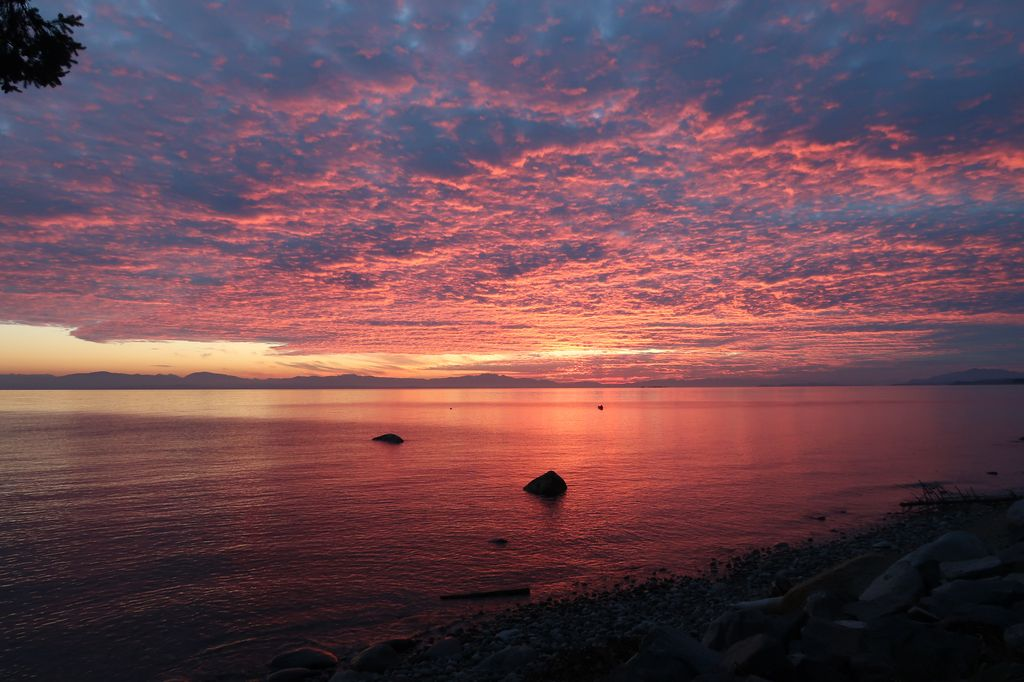
\includegraphics{images/20181016_coucher.JPG}
\caption{Coucher de soleil.}
\end{figure}

\begin{figure}
\centering
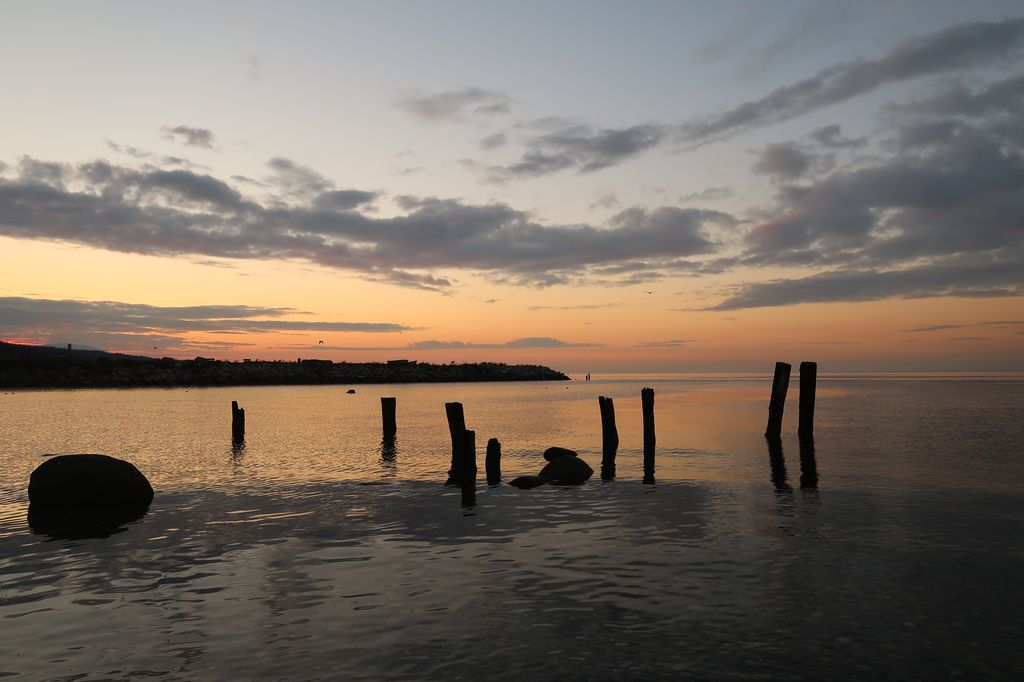
\includegraphics{images/20181016_lever.JPG}
\caption{Lever de soleil.}
\end{figure}

Avons-nous des regrets en partant, malgré notre séjour agréable à
Vancouver ? Eh bien oui ! Il se trouve que j'ai des parents très
éloignés de la famille Le Bourdais qui habitent en Colombie Britannique.
Surprise, ils font partie d'une tribu amérindienne, les \emph{Whispering
Pines / Clinton Indian Band}. Je les ai contacté pour les rencontrer,
mais nous n'avons finalement pas pris le temps d'aller les rencontrer.
Ce sera pour une autre fois.

L'autre regret sera celui de ne pas avoir pris quelques jours pour
explorer l'île de Vancouver. Si vaste que l'on pensait dans les premiers
temps de la découverte de l'Amérique que
\href{https://www.franceinter.fr/emissions/sur-les-epaules-de-darwin/sur-les-epaules-de-darwin-01-octobre-2016}{son
pourtour sud donnait accès au passage du Nord-Ouest}, j'aurai aimé y
admirer le
\href{https://fr.wikipedia.org/wiki/Cap_Flattery\#/media/File:CapeFlatteryWashington.jpg}{pilier
de Juan de Fuca}. Mais il aurait fallu passer la frontière des
Etats-Unis pour ça...

A tantôt pour de nouvelles aventures chez nos cousins québecois !

\emph{Florian}
